%%%%%%%%%%%%%%%
% This CV example/template is based on my own
% CV which I (lamely attempted) to clean up, so that
% it's less of an eyesore and easier for others to use.
%
% LianTze Lim (liantze@gmail.com)
% 23 Oct, 2022
%
\documentclass[a4paper,skipsamekey,11pt,english]{curve}
\makeatletter % <=======================================================
\def\@continuedname{}
\makeatother % <========================================================
% Default biblatex style used for the publication list is APA6. If you wish to use a different style or pass other options to biblatex you can change them here. 
\PassOptionsToPackage{style=ieee,sorting=ydnt,uniquename=init,defernumbers=true}{biblatex}

% Most commands and style definitions are in settings.sty.
\usepackage{settings}

% If you need to further customise your biblatex setup e.g. with \DeclareFieldFormat etc please add them here AFTER loading settings.sty. For example, to remove the default "[Online] Available:" prefix before URLs when using the IEEE style:
\DefineBibliographyStrings{english}{url={\textsc{url}}}

%% Only needed if you want a Publication List
\addbibresource{mypapers.bib}

%% Specify your last name(s) and first name(s) (as given in the .bib) to automatically bold your own name in the publications list. 
%% One caveat: You need to write \bibnamedelima where there's a space in your name for this to work properly; or write \bibnamedelimi if you use initials in the .bib
% \mynames{Lim/Lian\bibnamedelima Tze}

%% You can specify multiple names like this, especially if you have changed your name or if you need to highlight multiple authors. See items 6–9 in the example "Journal Articles" output.
%\mynames{Lim/Lian\bibnamedelima Tze,
%  Wong/Lian\bibnamedelima Tze,
%  Lim/Tracy,
%  Lim/L.\bibnamedelimi T.}
\mynames{Sharma\bibnamedelima Vatsalya,
            Sharma\bibnamedelima V.,
            Sharma/Vatsalya}
%% MAKE SURE THERE IS NO SPACE AFTER THE FINAL NAME IN YOUR \mynames LIST
\usepackage{comment}

% Change the fonts if you want
\ifxetexorluatex % If you're using XeLaTeX or LuaLaTeX
  \usepackage{fontspec} 
  %% You can use \setmainfont etc; I'm just using these font packages here because they provide OpenType fonts for use by XeLaTeX/LuaLaTeX anyway
  \usepackage[p,osf,swashQ]{cochineal}
  \usepackage[medium,bold]{cabin}
  \usepackage[varqu,varl,scale=0.9]{zi4}
\else % If you're using pdfLaTeX or latex
  \usepackage[T1]{fontenc}
  \usepackage[p,osf,swashQ]{cochineal}
  \usepackage{cabin}
  \usepackage[varqu,varl,scale=0.9]{zi4}
\fi

% Change the page margins if you want
% \geometry{left=1cm,right=1cm,top=1.5cm,bottom=1.5cm}

% Change the colours if you want
\definecolor{SwishLineColour}{HTML}{00FFFF}
\definecolor{MarkerColour}{HTML}{0000CC}

% Change the item prefix marker if you want
\prefixmarker{$\diamond$}

%% Photo is only shown if "fullonly" is included
\includecomment{fullonly}
% \excludecomment{fullonly}
%% ********************************  Add from here  <<<<<<<<<<<<<
\makeatletter
\renewenvironment{rubric}[1]{%
    \def\raggedright{%
        \@rightskip\@flushglue\rightskip\@rightskip\leftskip\z@skip}%
    \def\raggedleft{%
        \rightskip\z@skip\leftskip\@flushglue\parfillskip\z@skip}%
    \gdef\@beforespace{0pt}%
    \gdef\@nextentry{}%
    \gdef\@previouskey{}%
    \global\let\old@newpage\newpage%
    \global\let\old@pagebreak\pagebreak%
    \global\let\old@nopagebreak\nopagebreak
    \begin{longtable}{@{}kl@{~}X@{}}
        \@rubrichead{#1}\\*[\rubricspace]
        \endfirsthead
        \noalign{\@rubricmark{#1}%
            \global\let\in@newpage\newpage%
            \global\let\in@pagebreak\pagebreak%
            \global\let\in@nopagebreak\nopagebreak%
            \gdef\newpage{\@nextentry\noalign{\gdef\@nextentry{}}\in@newpage}
            \gdef\pagebreak{\@nextentry\noalign{\gdef\@nextentry{}}\in@pagebreak}
            \gdef\nopagebreak{\@nextentry\noalign{\gdef\@nextentry{}}\in@nopagebreak}}}{%
        \@nextentry
    \end{longtable}\par\vspace\rubricafterspace
    \global\let\newpage\old@newpage%
    \global\let\pagebreak\old@pagebreak%
    \global\let\nopagebreak\old@nopagebreak}
\makeatother
%%% *****************************************  TO HERE <<<<<<<<<<<<

%%%%%%%%%%%%%%%%%%%%%%%%%%%%%%%%%%%%%%

\begin{comment}
    

\leftheader{%
  {\LARGE\bfseries\sffamily Your Name Here, Ph.D.}

  \makefield{\faEnvelope[regular]}{\href{mailto:example@gmail.com}{\texttt{example@gmail.com}}}
  \makefield{\faTwitter}{\href{https://twitter.com/overleaf_example}{\texttt{@overleaf\_example}}}
  \makefield{\faLinkedin}
  {\href{http://www.linkedin.com/in/example/}{\texttt{example}}}

  %% Next line
  \makefield{\faGlobe}{\url{http://example.example.org/}}

  % You can use a tabular here if you want to line up the fields.
}

\rightheader{~}
\begin{fullonly}
\photo[r]{vatsalya.JPG}
\photoscale{0.25}
\end{fullonly}
\end{comment}
\title{Curriculum Vitae}

\begin{document}
\noindent \LARGE{\textbf{Vatsalya Sharma}}
\vspace{+1ex}
\hrule
\vspace{+2ex} 
\normalsize 
%\begin{minipage}[t]{0.05\textwidth}
%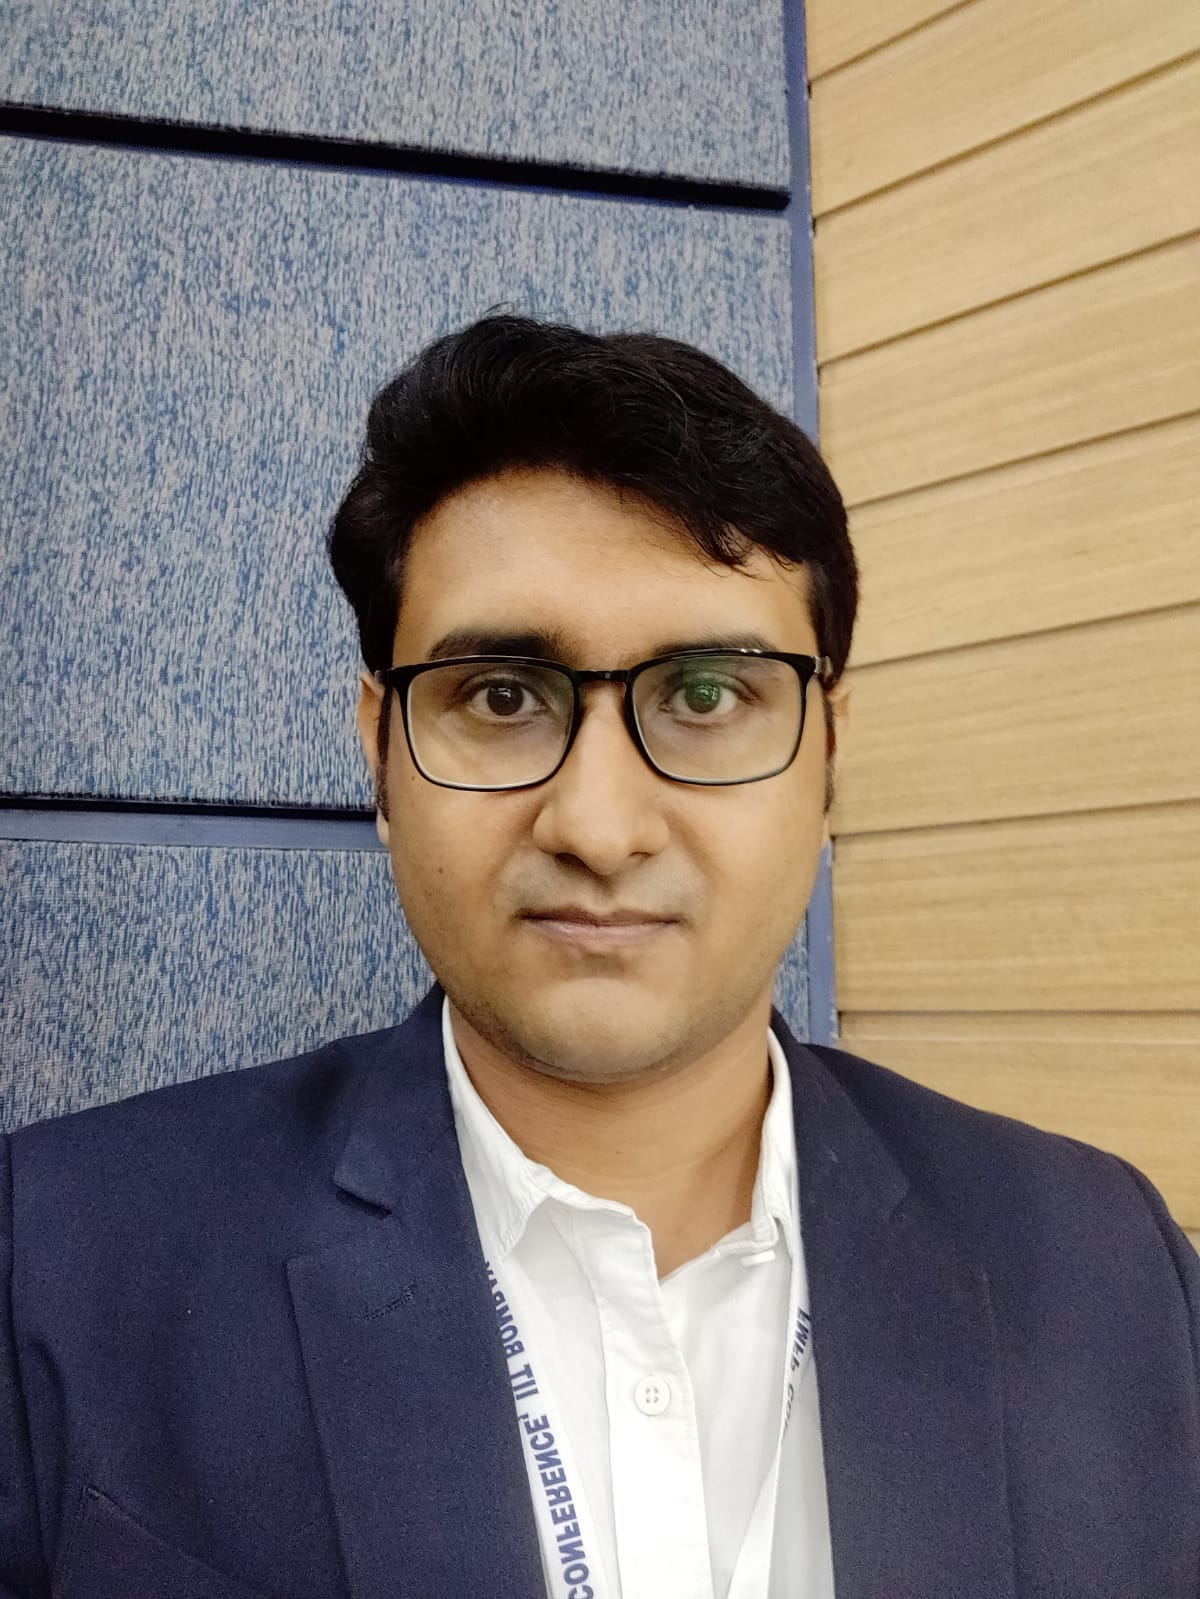
\includegraphics[trim={5cm 3cm 3cm 10cm},clip,scale=0.08]{vatsalya}
%\end{minipage}\hspace{0.1em}\hfill
%\begin{minipage}[t]{0.9\textwidth}
%\vspace{-8em}
\begin{minipage}[t]{0.7\textwidth} %without photo
\flushright
\begin{tabular}{l  | l }
 Postdoctoral Researcher, &   Scopus ID: 57191244967 \\
 KU Leuven,  &      ORCID: 0000-0003-2781-6563 \\
 Center for Mathematical Plasma Astrophysics,  &      \href{https://scholar.google.com/citations?user=lXGrvLoAAAAJ&hl=en}{Google Scholar} \\
 04.29, 200B Celestijenlaan,          &        \href{mailto:me12m1030@gmail.com}{me12m1030@gmail.com}  \\
 Leuven, Belgium 3001.  &      \href{mailto:vatsalya.sharma@kuleuven.be}{vatsalya.sharma@kuleuven.be}
\end{tabular}
\end{minipage}
\vspace{+1ex}
\hrule
\vspace{+2ex} 
%\makeheaders[c]
\makerubric{researchinterest}
\makerubric{ResearchExperience}
\makerubric{education}
%\makerubric{skills}
\makerubric{awards}
\makerubric{funding}
\makerubric{major_codes_developed}
\makerubric{teaching_experience}
\makerubric{employment}
\makerubric{collaborations}
\makerubric{journal_reviewer}
\makerubric{activities}

%campus dept talks
% If you're not a researcher nor an academic, you probably don't have any publications; delete this line.
%% Sometimes when a section can't be nicely modelled with the \entry[]... mechanism; hack our own and use \input NOT \makerubric
\newpage
\makerubric{courses}
%% Sometimes when a section can't be nicely modelled with the \entry[]... mechanism; hack our own
%\newpage
\makerubrichead{Research Publications}

%% Assuming you've already given \addbibresource{own-bib.bib} in the main doc. Right? Right???
\nocite{*}

%% If you just want everything in one list
% \printbibliography[heading={none}]

\printbibliography[heading={subbibliography},title={Journal Articles},type=article]
%\newpage
\printbibliography[heading={subbibliography},title={Under Review},type=misc]

\printbibliography[heading={subbibliography},title={Conference Proceedings},type=inproceedings]

\printbibliography[heading={subbibliography},title={Books and Chapters},filter={booksandchapters}]



%\makerubric{referee}
%\newpage
%% Probably not the best way of doing it but what the heck, I just winged-it :p
%\newpage
\makerubrichead{References}

\begin{tabularx}{\textwidth}{@{}X X@{}}
\textbf{Prof Vinayak Eswaran} (thesis advisor)\par
Professor,\par
Mechanical and Aerospace Engineering Department,\par 
Indian Institute of Technology Hyderabad, India.\par 
\makefield{\faEnvelopeO}{\url{eswar@mae.iith.ac.in}}
& 
\textbf{Prof Debasis Chakraborty} (thesis co-advisor)\par
Professor,\par
Mechanical Engineering Department,\par 
Mahindra University, Hyderabad, Telangana, India.\par 
\makefield{\faEnvelopeO}{\url{debasisc.cfd@gmail.com}}
\\
\\
%\textbf{Dr. Andrea Lani} (Postdoctoral research promoter)\par
%Research Manager, \par
%at KU Leuven and,\par 
%Von-Karmann Institute of Fluid Dynamics, Belgium.\par 
%\makefield{\faEnvelopeO}{\url{andrea.lani@kuleuven.be}}
\textbf{Dr. Andrea Lani} (Postdoctoral research promoter)\par
Research Manager, \par
Center for Mathematical Plasma Astrophysics, \par
KU Leuven, Belgium.\par 
%Von-Karmann Institute of Fluid Dynamics, Belgium.\par 
\makefield{\faEnvelopeO}{\url{andrea.lani@kuleuven.be}}
%& 
%\textbf{Prof. Abhay Sharma } (Collaborator)\par
%Professor,\par
%Department of Mechanical Engineering,\par 
%Indian Institute of Technology Jammu.\par 
%\makefield{\faEnvelopeO}{\url{abhay.sharma@iitjammu.ac.in}}
%& 
%\textbf{Prof. Stefaan Poedts } (PDF co-promoter)\par
%Professor,\par
%Center for Mathematical Plasma Astrophysics,\par 
%KU Leuven, Belgium.\par 
%\makefield{\faEnvelopeO}{\url{stefaan.poedts@kuleuven.be}}
%\\


%\textbf{Prof. Abhay Sharma } (Collaborator)\par
%Professor,\par
%Department of Materials Engineering,\par 
%KU Leuven, Belgium.\par 
%\makefield{\faEnvelopeO}{\url{abhay.sharma@kuleuven.be}}
%& 
%\textbf{Dr. Ashwani Assam} (Collaborator)\par
%Assistant Professor,\par
%Mechanical Engineering Department,\par 
%Indian Institute of Technology Patna, India.\par 
%\makefield{\faEnvelopeO}{\url{aashwani@iitp.ac.in}}
\end{tabularx}

\end{document}